\section{Experimental results} 
We now describe the experimentations conducted to verify the correctness of the features extracted from \emph{SeedsAnalyser} using the classification plugin.
We selected the images containing the most numerous samples per species from the \emph{Fabaceae} database, for a total of 23 different ones: 
\emph{Amorpha}, \emph{Anagyris}, \emph{Anthyllis barba jovis}, \emph{Anthyllis cytisoides}, \emph{Astragalus glycyphyllos}, \emph{Calicotome}, \emph{Caragana}, \emph{Ceratonia}, \emph{Colutea}, \emph{Cytisus purgans}, \emph{Cytisus scoparius}, \emph{Dorycnium pentaphyllum}, \emph{Dorycnium rectum}, \emph{Hedysarum coronarium}, \emph{Lathyrus aphaca}, \emph{Lathyrus ochrus}, \emph{Medicago sativa}, \emph{Melilotus officinalis}, \emph{Pisum}, \emph{Senna alexandrina}, \emph{Spartium junceum}, \emph{Trifolium}, \emph{Vicia faba}, for a total of 1988 seeds.
A sample of each species is shown in Figure \ref{Sardinia_samples}, while Table \ref{Sardinia_tab} reports the number of samples for each species.

\begin{figure}[htbp]
	\centering
	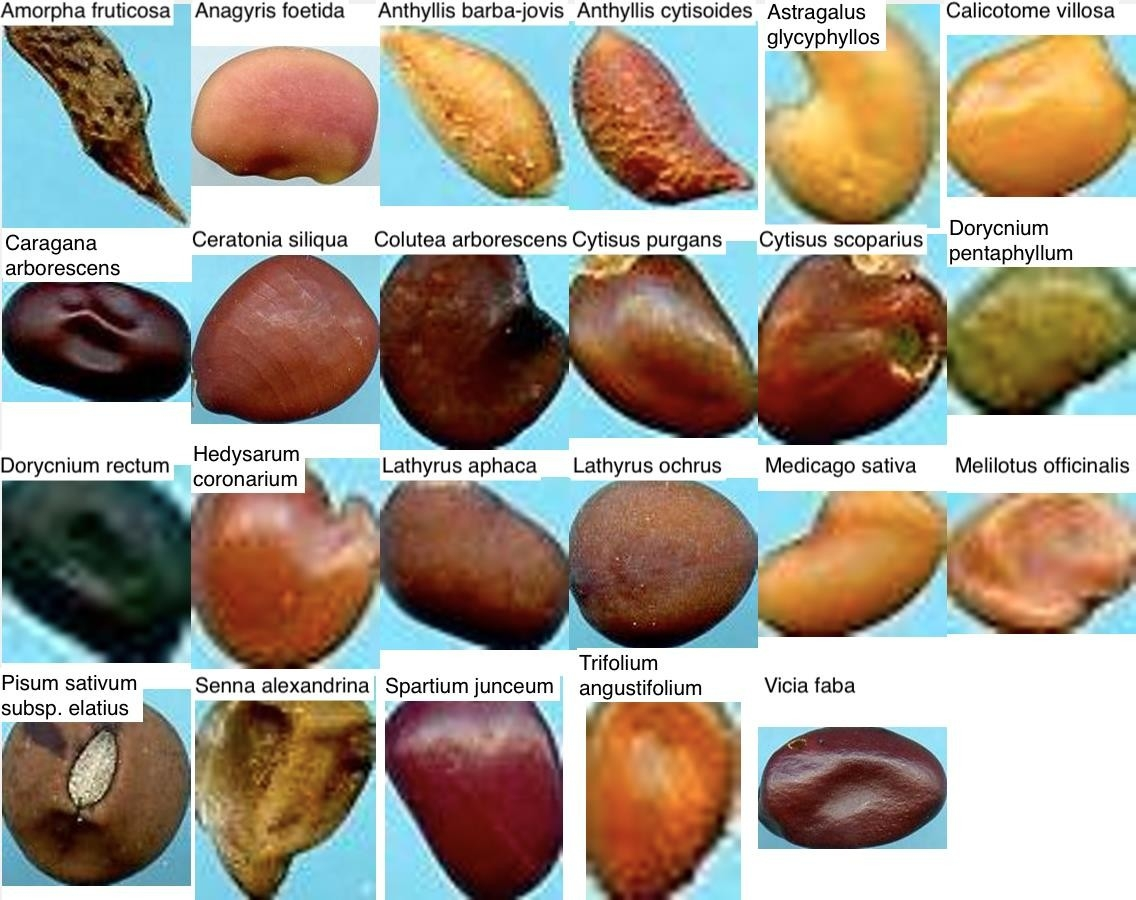
\includegraphics[scale=0.65]{Sardinia_samples.jpg}
	\caption{A sample of seed for each species present in the \emph{Fabaceae} dataset.}
	\label{Sardinia_samples}
\end{figure}

\begin{table}[htbp]
	\centering
	\small
	\hspace{0.05cm}
	\begin{tabular}{lc}
		\hline
		\textbf{Species} & \textbf{Num. of samples} \\
		\hline
		\emph{Amorpha} & 51 \\
		\emph{Anagyris} & 29 \\
		\emph{Anthyllis barba jovis} & 51 \\
		\emph{Anthyllis cytisoides} & 29 \\
		\emph{Astragalus glycyphyllos} & 50 \\
		\emph{Calicotome} & 32 \\
		\emph{Caragana} & 36 \\
		\emph{Ceratonia} & 45 \\
		\emph{Colutea} & 42 \\
		\emph{Cytisus purgans} & 44 \\
		\emph{Cytisus scoparius} & 65 \\
		\emph{Dorycnium pentaphyllum} & 42 \\
		\emph{Dorycnium rectum} & 236 \\
		\emph{Hedysarum coronarium} & 208 \\
		\emph{Lathyrus aphaca} & 52 \\
		\emph{Lathyrus ochrus} & 46 \\
		\emph{Medicago sativa} & 116 \\
		\emph{Melilotus officinalis} & 176 \\
		\emph{Pisum} & 121 \\
		\emph{Senna alexandrina} & 194 \\
		\emph{Spartium junceum} & 109  \\
		\emph{Trifolium} & 183 \\
		\emph{Vicia faba} & 31 \\
		\hline
	\end{tabular}
	\caption{\emph{Fabaceae} dataset description.} 
	\label{Sardinia_tab}
\end{table}

As described in Sec. \ref{seeds_analyser} we have implemented and extracted three categories of handcrafted features from the seeds: morphological structure, texture information, and colour intensity values, for a total amount of 64 descriptors. Afterwards, we provided them as inputs to four different classification models, namely kNN, Naive Bayes, Random Forest, and Support Vector Machine, using our plugin \emph{SeedsClassifier}, based on Weka package tool \cite{Weka}. 

To ensure training set heterogeneity, we trained each classifier with 10-fold cross-validation, and for each case, we selected the model with the largest area under the ROC curve (AUC). 

The performance measures used to quantify each classification model's performance are specificity, sensitivity, and accuracy. 
The specificity (Spec) measures the proportion of negatives that are correctly identified (also called true negative rate). The sensitivity (Sen) measures the proportion of positives that are correctly identified (also called true positive rate).
The third measure is the accuracy (Acc), defined as the correctly labelled instances' ratio to the whole pool of instances. 
Finally, as we face a multi-class imbalanced problem, we also applied three of the most common global metrics for multi-class imbalance learning to evaluate the classifier's performance \cite{Alejo2013}. The used measures are the macro average geometric (MAvG), defined as the geometric average of the partial accuracy of each class, the mean F-measure (MFM) and the macro average arithmetic (MAvA), defined as the arithmetic average of the partial accuracies of each class. 

We performed several experiments for each classifier. In particular, we tested the descriptors categories both alone and in combination with the others to understand if there is the best descriptor category for this task. Finally, we use the \emph{SeedsClassifier} plugin to classify each category with the chosen classifiers.

Tables \ref{Table_classification_kNN}, \ref{Table_classification_Bayes}, \ref{Table_classification_RF}, \ref{Table_classification_SVM} show all the classification results on the analysed dataset.
In detail, the kNN classifier shows high results with colour features category alone, outperforming the remaining. Surprisingly, the combination of all categories does not reach the best metric results with this classifier.
Random Forest classifier substantially confirms the trend brought by the colour feature category. It outperforms every other combination, even against the remaining classifiers. However, the combination of all categories produced excellent results with the Random Forest model.
Naive Bayes and SVM classifiers produced satisfactory results using all categories, which results in the best one for both classifiers. Contrary to kNN and Random Forest results, the colour category alone did not produce good results in these last two cases.
To sum up, the Random Forest classifier produced the best performance and is the only one to exceed 90\% both in metrics and in categories combination. It confirms its outstanding versatility in this twenty-three-class scenario. 
Finally, we can say that combining all the three feature categories produces excellent results in most cases and satisfactory on average.

\begin{table}[htbp]
	\centering
	\caption{Results using every possible combination of classic descriptors and kNN.}
	\label{Table_classification_kNN}
	\begin{tabular}{lcccccc}
		\toprule
		Descriptors    &  Acc  & Spec  &  Sen  & MAvG  &  MFM  & MAvA  \\ \midrule
		Morphological & 20.95 & 23.18 & 17.10 & 9.94 & 18.59 & 23.18 \\
		Texture & 16.41 & 20.52 & 16.97 & 10.91 & 16.36 & 20.52 \\
		Colour & 80.54 & 76.59 & 74.70 & 74.72 & 75.15 & 76.59 \\
		Morphological+Texture & 31.25 & 27.57 & 22.17 & 13.73 & 23.62 & 27.57 \\
		Morphological+Colour & 45.13 & 41.63 & 33.47 & 27.08 & 35.34 & 41.63 \\
		Texture+Colour & 68.61 & 62.33 & 58.44 & 57.74 & 59.73 & 62.33 \\
		All & 71.68 & 69.54 & 63.02 & 65.60 & 65.17 & 69.54 \\ \bottomrule
	\end{tabular}
\end{table}

\begin{table}[htbp]
	\centering
	\caption{Results using every possible combination of classic descriptors and Naive Bayes.}
	\label{Table_classification_Bayes}
	\begin{tabular}{lcccccc}
		\toprule
		Descriptors    &  Acc  & Spec  &  Sen  & MAvG  &  MFM  & MAvA  \\ \midrule
		Morphological & 62.42 & 59.88 & 62.04 & 53.34 & 59.68 & 59.88 \\
		Texture & 48.19 & 47.59 & 45.84 & 39.58 & 43.43 & 47.59 \\
		Colour & 65.21 & 60.75 & 62.25 & 55.02 & 57.93 & 60.75 \\
		Morphological+Texture & 76.81 & 73.00 & 75.10 & 68.51 & 72.89 & 73.00 \\
		Morphological+Colour & 84.36 & 81.66 & 84.43 & 79.22 & 82.35 & 81.66 \\
		Texture+Colour & 79.33 & 76.14 & 79.15 & 72.81 & 75.74 & 76.14 \\ 
		All & 85.16 & 81.78 & 84.82 & 79.68 & 82.76 & 81.78 \\ \bottomrule
	\end{tabular}
\end{table}

\begin{table}[htbp]
	\centering
	\captionsetup{width=.9\textwidth}
	\caption{Results using every possible combination of classic descriptors and Random Forest.}
	\label{Table_classification_RF}
	\begin{tabular}{lcccccc}
		\toprule
		Descriptors    &  Acc  & Spec  &  Sen  & MAvG  &  MFM  & MAvA  \\ \midrule
		Morphological & 40.48 & 46.85 & 29.13 & 37.96 & 27.58 & 46.85 \\
		Texture & 72.03 & 65.88 & 60.38 & 62.09 & 61.17 & 65.88 \\
		Colour & 94.27 & 94.85 & 91.05 & 94.67 & 92.52 & 94.85 \\
		Morphological+Texture & 89.64 & 90.67 & 81.96 & 90.09 & 83.79 & 90.67 \\
		Morphological+Colour & 92.71 & 93.57 & 88.94 & 93.36 & 90.67 & 93.57 \\
		Texture+Colour & 92.05 & 92.41 & 87.16 & 92.21 & 89.07 & 92.41 \\ 
		All & 93.76 & 94.55 & 89.75 & 94.37 & 91.39 & 94.55 \\ \bottomrule
	\end{tabular}
\end{table}

\begin{table}[htbp]
	\centering
	\caption{Results using every possible combination of classic descriptors and SVM.}
	\label{Table_classification_SVM}
	\begin{tabular}{lcccccc}
		\toprule
		Descriptors    &  Acc  & Spec  &  Sen  & MAvG  &  MFM  & MAvA  \\ \midrule
		Morphological & 79.83 & 80.26 & 71.33 & 79.46 & 73.23 & 80.26 \\
		Texture & 29.09 & 46.28 & 21.13 & 34.11 & 16.91 & 46.28 \\
		Colour & 78.74 & 75.28 & 67.83 & 72.42 & 67.88 & 75.28 \\
		Morphological+Texture & 66.05 & 59.81 & 51.10 & 52.83 & 52.44 & 59.81 \\
		Morphological+Colour & 83.60 & 83.10 & 76.70 & 81.65 & 78.88 & 83.10 \\
		Texture+Colour & 84.51 & 84.99 & 77.73 & 84.15 & 78.81 & 84.99 \\
		All & 85.66 & 83.85 & 78.88 & 82.56 & 80.58 & 83.85 \\ \bottomrule
	\end{tabular}
\end{table}